\begin{figure}[H]
    \centering
\tikzset{every picture/.style={line width=0.75pt}} %set default line width to 0.75pt        

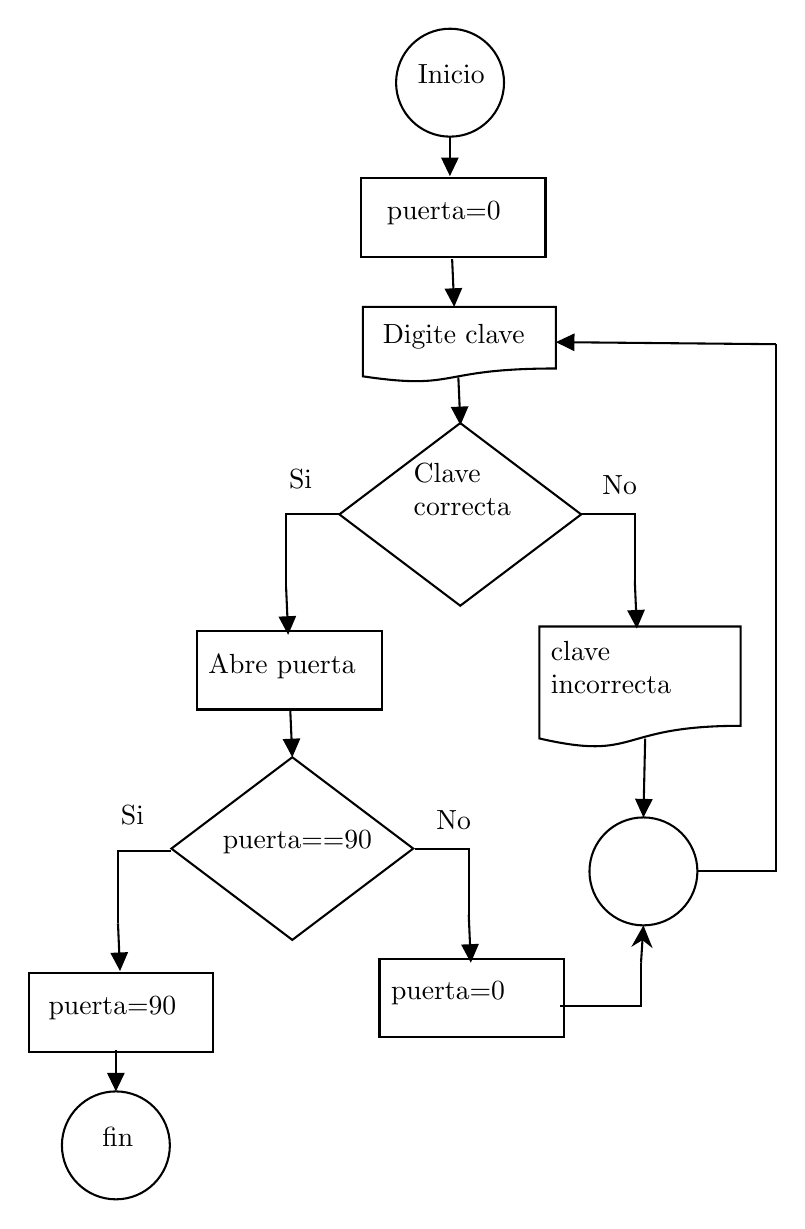
\begin{tikzpicture}[x=0.75pt,y=0.75pt,yscale=-1,xscale=1]
%uncomment if require: \path (0,649); %set diagram left start at 0, and has height of 649

%Flowchart: Connector [id:dp42585090626324207] 
\draw   (304,59) .. controls (304,44.64) and (315.64,33) .. (330,33) .. controls (344.36,33) and (356,44.64) .. (356,59) .. controls (356,73.36) and (344.36,85) .. (330,85) .. controls (315.64,85) and (304,73.36) .. (304,59) -- cycle ;
%Straight Lines [id:da9927818650372262] 
\draw    (329.92,85) -- (329.92,101) ;
\draw [shift={(329.92,104)}, rotate = 270] [fill={rgb, 255:red, 0; green, 0; blue, 0 }  ][line width=0.08]  [draw opacity=0] (8.93,-4.29) -- (0,0) -- (8.93,4.29) -- cycle    ;
%Flowchart: Decision [id:dp8222109791046812] 
\draw   (334.92,223) -- (393.17,267) -- (334.92,311) -- (276.67,267) -- cycle ;
%Shape: Right Angle [id:dp5468713947182464] 
\draw   (276.67,267) -- (251,267) -- (251,302) ;
%Straight Lines [id:da34123972616362797] 
\draw    (251,302) -- (251.87,322) ;
\draw [shift={(252,325)}, rotate = 267.51] [fill={rgb, 255:red, 0; green, 0; blue, 0 }  ][line width=0.08]  [draw opacity=0] (8.93,-4.29) -- (0,0) -- (8.93,4.29) -- cycle    ;
%Flowchart: Process [id:dp6422094052668206] 
\draw   (208,323) -- (297,323) -- (297,361) -- (208,361) -- cycle ;
%Shape: Right Angle [id:dp9632380337734168] 
\draw   (393.17,267) -- (419,267) -- (419,299) ;
%Straight Lines [id:da9224648988654192] 
\draw    (419,299) -- (419.87,319) ;
\draw [shift={(420,322)}, rotate = 267.51] [fill={rgb, 255:red, 0; green, 0; blue, 0 }  ][line width=0.08]  [draw opacity=0] (8.93,-4.29) -- (0,0) -- (8.93,4.29) -- cycle    ;
%Straight Lines [id:da14093121348085114] 
\draw    (424,375) -- (423.23,410) ;
\draw [shift={(423.17,413)}, rotate = 271.26] [fill={rgb, 255:red, 0; green, 0; blue, 0 }  ][line width=0.08]  [draw opacity=0] (8.93,-4.29) -- (0,0) -- (8.93,4.29) -- cycle    ;
%Flowchart: Connector [id:dp28231580529895073] 
\draw   (143,571) .. controls (143,556.64) and (154.64,545) .. (169,545) .. controls (183.36,545) and (195,556.64) .. (195,571) .. controls (195,585.36) and (183.36,597) .. (169,597) .. controls (154.64,597) and (143,585.36) .. (143,571) -- cycle ;
%Flowchart: Document [id:dp7887811718871025] 
\draw   (373,321) -- (470,321) -- (470,368.85) .. controls (409.38,368.85) and (421.5,386.1) .. (373,374.94) -- cycle ;
%Shape: Right Angle [id:dp7465732461480319] 
\draw   (449.17,439) -- (487,439) -- (487,185) ;
%Straight Lines [id:da9427213356074324] 
\draw    (384,184.03) -- (487,185) ;
\draw [shift={(381,184)}, rotate = 0.54] [fill={rgb, 255:red, 0; green, 0; blue, 0 }  ][line width=0.08]  [draw opacity=0] (8.93,-4.29) -- (0,0) -- (8.93,4.29) -- cycle    ;
%Flowchart: Connector [id:dp6793358076053446] 
\draw   (397.17,439) .. controls (397.17,424.64) and (408.81,413) .. (423.17,413) .. controls (437.53,413) and (449.17,424.64) .. (449.17,439) .. controls (449.17,453.36) and (437.53,465) .. (423.17,465) .. controls (408.81,465) and (397.17,453.36) .. (397.17,439) -- cycle ;
%Straight Lines [id:da6157101498528812] 
\draw    (253,361) -- (253.87,381) ;
\draw [shift={(254,384)}, rotate = 267.51] [fill={rgb, 255:red, 0; green, 0; blue, 0 }  ][line width=0.08]  [draw opacity=0] (8.93,-4.29) -- (0,0) -- (8.93,4.29) -- cycle    ;
%Flowchart: Process [id:dp10984865947746725] 
\draw   (296,481) -- (385,481) -- (385,519) -- (296,519) -- cycle ;
%Flowchart: Process [id:dp2789359345260862] 
\draw   (287,105) -- (376,105) -- (376,143) -- (287,143) -- cycle ;
%Straight Lines [id:da14083283346218511] 
\draw    (334,201) -- (334.87,221) ;
\draw [shift={(335,224)}, rotate = 267.51] [fill={rgb, 255:red, 0; green, 0; blue, 0 }  ][line width=0.08]  [draw opacity=0] (8.93,-4.29) -- (0,0) -- (8.93,4.29) -- cycle    ;
%Flowchart: Decision [id:dp06088544865395984] 
\draw   (254,384) -- (312.25,428) -- (254,472) -- (195.75,428) -- cycle ;
%Shape: Right Angle [id:dp8217099184396621] 
\draw   (313.17,428) -- (339,428) -- (339,460) ;
%Straight Lines [id:da965375327404175] 
\draw    (339,460) -- (339.87,480) ;
\draw [shift={(340,483)}, rotate = 267.51] [fill={rgb, 255:red, 0; green, 0; blue, 0 }  ][line width=0.08]  [draw opacity=0] (8.93,-4.29) -- (0,0) -- (8.93,4.29) -- cycle    ;
%Shape: Right Angle [id:dp7886934725142394] 
\draw   (195.67,429) -- (170,429) -- (170,464) ;
%Straight Lines [id:da8518021831322284] 
\draw    (170,464) -- (170.87,484) ;
\draw [shift={(171,487)}, rotate = 267.51] [fill={rgb, 255:red, 0; green, 0; blue, 0 }  ][line width=0.08]  [draw opacity=0] (8.93,-4.29) -- (0,0) -- (8.93,4.29) -- cycle    ;
%Flowchart: Process [id:dp8640224184714345] 
\draw   (127,488) -- (216,488) -- (216,526) -- (127,526) -- cycle ;
%Shape: Right Angle [id:dp5762038720241354] 
\draw   (383,504) -- (422,504) -- (422,483) ;
%Straight Lines [id:da6437862550472608] 
\draw    (422,483) -- (422.97,467.99) ;
\draw [shift={(423.17,465)}, rotate = 93.71] [fill={rgb, 255:red, 0; green, 0; blue, 0 }  ][line width=0.08]  [draw opacity=0] (10.72,-5.15) -- (0,0) -- (10.72,5.15) -- (7.12,0) -- cycle    ;
%Flowchart: Document [id:dp3979180887556457] 
\draw   (288,167) -- (381,167) -- (381,196.7) .. controls (322.88,196.7) and (334.5,207.41) .. (288,200.48) -- cycle ;
%Straight Lines [id:da5018025676967481] 
\draw    (331,144) -- (331.87,164) ;
\draw [shift={(332,167)}, rotate = 267.51] [fill={rgb, 255:red, 0; green, 0; blue, 0 }  ][line width=0.08]  [draw opacity=0] (8.93,-4.29) -- (0,0) -- (8.93,4.29) -- cycle    ;
%Straight Lines [id:da6767101156206579] 
\draw    (169,525) -- (169,542) ;
\draw [shift={(169,545)}, rotate = 270] [fill={rgb, 255:red, 0; green, 0; blue, 0 }  ][line width=0.08]  [draw opacity=0] (8.93,-4.29) -- (0,0) -- (8.93,4.29) -- cycle    ;

% Text Node
\draw (313,49) node [anchor=north west][inner sep=0.75pt]   [align=left] {Inicio};
% Text Node
\draw (250.92,244) node [anchor=north west][inner sep=0.75pt]   [align=left] {Si};
% Text Node
\draw (212.08,332.67) node [anchor=north west][inner sep=0.75pt]   [align=left] {Abre puerta};
% Text Node
\draw (311,241) node [anchor=north west][inner sep=0.75pt]   [align=left] {Clave\\correcta\\};
% Text Node
\draw (401.92,247) node [anchor=north west][inner sep=0.75pt]   [align=left] {No};
% Text Node
\draw (161,561) node [anchor=north west][inner sep=0.75pt]   [align=left] {fin};
% Text Node
\draw (377.08,326.67) node [anchor=north west][inner sep=0.75pt]   [align=left] {clave\\incorrecta};
% Text Node
\draw (300.08,490.67) node [anchor=north west][inner sep=0.75pt]   [align=left] {puerta=0};
% Text Node
\draw (298.08,114.67) node [anchor=north west][inner sep=0.75pt]   [align=left] { puerta=0};
% Text Node
\draw (219,418) node [anchor=north west][inner sep=0.75pt]   [align=left] {puerta==90};
% Text Node
\draw (321.92,408) node [anchor=north west][inner sep=0.75pt]   [align=left] {No};
% Text Node
\draw (169.92,406) node [anchor=north west][inner sep=0.75pt]   [align=left] {Si};
% Text Node
\draw (135.08,497.67) node [anchor=north west][inner sep=0.75pt]   [align=left] {puerta=90};
% Text Node
\draw (296.08,173.67) node [anchor=north west][inner sep=0.75pt]   [align=left] {Digite clave};


\end{tikzpicture}

    \caption{Diagrama de bloques smart door lock.}
    \label{sch_1}
\end{figure}